\documentclass{article}

\usepackage[preprint]{neurips_2025}
\usepackage[utf8]{inputenc}
\usepackage[T1]{fontenc}
\usepackage{booktabs}
\usepackage{amsmath}
\usepackage{graphicx}
\usepackage{hyperref}
\usepackage{url}
\usepackage{array}
\usepackage{multirow}
\usepackage{tabularx}

\graphicspath{{../outputs/figures/}}

\title{Predicting the 2026 FIFA World Cup: A Full Project Report Across Match Outcome Models}

\author{%
  Taha Ahmad \\
  \And
  Ilir Bejleri \\
  \And
  Ahmed Alamin \\
}

\begin{document}
\maketitle
\begin{center}
  \small Code repository:
  \url{https://github.com/ilirbejleri/world-cup-ml-final}
\end{center}

\begin{abstract}
This project builds an end-to-end machine learning system for FIFA World Cup
prediction. The pipeline is self-contained in the
\texttt{final/} directory \citep{worldcupmlrepo} and converts cached historical football data into
14,881 chronological supervised match examples: 964 World Cup rows and 13,917
other international fixtures. Every feature is computed before kickoff. Every
model is selected through walk-forward World Cup checkpoints: train on all
matches available before a World Cup, validate on that next tournament, and
repeat this for every feasible pre-2022 World Cup from 1938 through 2018. The
2022 World Cup is held out as the final test. We compare original MLR feature
sets, expanded MLR/RF/NN variants, independent Poisson score models,
draw-inflated Poisson models, and a validation-tuned ensemble. The best
held-out log loss is achieved by an 18-feature neural network using all
original engineered feature families (0.9321 on 2022). The best held-out
accuracy is achieved by a 53-feature NN ablation that removes the two noisiest
underdog-history features (60.9\% accuracy, 0.9363 log loss, and 30\% draw
recall). A classifier-calibrated Poisson score simulator powers the 5,000-run
2026 tournament forecast: the best log-loss NN supplies W/D/L probabilities,
and the score layer supplies calibrated goal counts. The project shows that
supervised international matches are necessary for high-capacity models. For
the 2026 forecast, the pipeline updates Elo, form, the outcome model, and the
score layer with 4,358 supplemental matches from 2022 through March 2026; Spain
has the highest simulated champion probability at 14.9\%.
\end{abstract}

\section{Introduction}

The FIFA World Cup is an attractive machine learning problem because it is
global, high-stakes, and structured, but it is also a difficult prediction
target. A modern tournament has only 64 matches before 2026, and the expanded
2026 tournament still has far fewer observations than ordinary supervised ML
settings. Football is also low scoring: a model can correctly identify the
stronger team and still miss a draw, penalty shootout, or single-goal upset.
For this project, accuracy and log loss both matter. Accuracy measures whether
the model selects the right outcome; log loss measures whether its probability
distribution is useful for simulation.

The central data-design choice is to treat international matches as supervised
labels rather than only as rating-history updates. Every international match in
the cache is a supervised example, while World Cup matches receive higher
sample weights so the target remains tournament behavior. The report describes
the complete system: data construction, engineered features, MLR/RF/NN/Poisson
comparisons, validation checkpoints, error analysis, and a 2026 tournament
forecast.

The project has four goals. First, compare multiple model families under one
leakage-resistant chronological protocol. Second, show exactly how the 18
engineered feature families are represented and how many each model uses.
Third, produce at least one strong high-accuracy model and one low-log-loss
probabilistic model. Fourth, use a hybrid outcome/score simulator to forecast
the configured 2026 World Cup field.

\section{Background}

Each match is represented from the perspective of the pre-match higher-Elo
team. The labels are Win, Draw, and Loss for that stronger side, so a Loss is
an upset. This framing avoids dependence on arbitrary home/away ordering in
neutral-site tournaments. Log loss is
\[
  \mathrm{LL} = -\frac{1}{N}\sum_{i=1}^{N}\log \hat p_{i,y_i},
\]
where $\hat p_{i,y_i}$ is the predicted probability assigned to the true
class. Log loss is the primary calibration metric because tournament
simulation uses probabilities rather than only argmax outcomes.

The model families reflect different assumptions. Multinomial logistic
regression (MLR) is a stable softmax baseline. Random forests (RF) capture
nonlinear feature interactions but can be less calibrated on small validation
sets \citep{breiman2001random}. Neural networks (NNs) can combine many
rolling-window signals but require enough supervised examples. Poisson score
models directly predict goals and derive win/draw/loss probabilities from a
score grid, following classical football score modeling
\citep{maher1982modelling,dixon1997modelling}. Elo ratings are used because
they have been shown to be useful in association-football prediction
\citep{hvattum2010using}.

\section{Setting}

\paragraph{Data.}
The final directory includes the raw match cache, feature code, report source,
style file, and bibliography. The supervised table contains 14,881 matches.
The base cache ends with internationals through 2021 and the 2022 World Cup.
Those rows are used for model comparison and 2022 testing. For the 2026
forecast only, we add a bundled supplemental international-results file
covering 2022 through March 2026 \citep{martj42international}. Table
\ref{tab:data} summarizes the base splits.

\begin{table}[ht]
\centering
\small
\caption{Final supervised dataset. International rows are training labels, not
only rating-history updates.}
\label{tab:data}
\begin{tabular}{lrrrr}
\toprule
Split & Rows & World Cup & International & Dates \\
\midrule
All supervised rows & 14,881 & 964 & 13,917 & 1930-07-13 to 2022-12-18 \\
Pre-2022 training pool & 14,817 & 900 & 13,917 & 1930-07-13 to 2021-12-31 \\
Held-out 2022 World Cup & 64 & 64 & 0 & 2022-11-20 to 2022-12-18 \\
\bottomrule
\end{tabular}
\end{table}

\paragraph{Walk-forward checkpoints.}
The validation protocol uses every feasible World Cup checkpoint before 2022.
For a checkpoint year $Y$, models train on matches before the first
match of World Cup $Y$ and validate on World Cup $Y$. Checkpoints begin in
1938 because 1934 lacks all three classes in the prior training data. The
final 2022 World Cup remains untouched until the end. This design directly
answers the assignment requirement that training on a set of matches be
tested on the next upcoming World Cup repeatedly.

\begin{table}[ht]
\centering
\small
\caption{Checkpoint protocol. Full per-model rows are written to
\texttt{outputs/fold\_metrics.csv}.}
\label{tab:folds}
\begin{tabular}{lrrr}
\toprule
Checkpoint range & WCs & First train rows & Last train rows \\
\midrule
1938--2018 validation & 19 & 35 & 12,551 \\
2022 final test & 1 & 14,817 & 14,817 \\
\bottomrule
\end{tabular}
\end{table}

\section{Methodology}

\paragraph{Chronological features and weights.}
A feature tracker processes matches in date order. For each row it records
pre-match Elo, rolling form, goals scored, goals conceded, clean sheets,
opponent strength, head-to-head history, World Cup history, and match context
before updating state with the result. World Cup rows receive base weight 5.0,
other internationals receive base weight 0.75, and both receive a 12-year
half-life decay:
\[
  w_i = w_{\mathrm{competition}(i)}\cdot 0.5^{(Y-y_i)/12}.
\]
This prevents old matches and lower-importance friendlies from overwhelming
the tournament target.

\paragraph{Eighteen engineered feature families.}
The feature design is organized around 18 engineered families.
Table~\ref{tab:features18} shows the families; the appendix contains the full
glossary. A is the higher-Elo team before kickoff, and B is the lower-Elo team.

\begin{table}[ht]
\centering
\small
\caption{Original engineered feature families used for model accounting.}
\label{tab:features18}
\begin{tabularx}{\textwidth}{lX}
\toprule
Family & Features \\
\midrule
Team strength & \texttt{elo\_a}, \texttt{elo\_b}, \texttt{wc\_hist\_a}, \texttt{wc\_hist\_b} \\
Recent form and scoring & \texttt{wr\_a}, \texttt{wr\_b}, \texttt{gd\_a}, \texttt{gd\_b}, \texttt{gs\_a}, \texttt{gs\_b} \\
Schedule and defense & \texttt{opp\_elo\_a}, \texttt{opp\_elo\_b}, \texttt{cs\_a}, \texttt{cs\_b} \\
Matchup and context & \texttt{h2h\_a}, \texttt{stage\_ord}, \texttt{upset\_a}, \texttt{gk\_b} \\
\bottomrule
\end{tabularx}
\end{table}

\paragraph{How 18 becomes 55.}
The 55-column full models are not 55 unrelated ideas. They expand the 18
families into multiple time windows and interaction terms. The strength block
contains eight columns: raw Elo for A/B, Elo difference, Elo win probability,
World Cup history for A/B, and recent opponent strength for A/B. Thus the
column count is explicit: $8+12+12+12+11=55$. Recent form
is expanded into three windows: last 5 matches, last 10 matches, and recent
4-year form. Each window includes win rate, goal differential, goals scored,
goals conceded, clean-sheet rate, and differences between A and B. Context
adds head-to-head features, stage indicators, World Cup indicators, absolute
strength gaps, squared Elo gap, and two underdog-history exponential moving
averages (EMAs): favorite-upset rate and underdog giant-killing rate. The
exact mapping is saved in \texttt{outputs/feature\_blocks\_55.csv}.

\begin{table}[ht]
\centering
\small
\caption{The 55 direct full-model columns are grouped into five blocks.}
\label{tab:blocks55}
\begin{tabular}{lrr}
\toprule
Block & Columns & Purpose \\
\midrule
Strength/history & 8 & Long-run team quality and tournament history \\
Last-5 form & 12 & Short-term performance and opponent quality \\
Last-10 form & 12 & More stable medium-window form \\
Recent 4-year form & 12 & Cycle-aware national-team form \\
Context/interactions & 11 & Stage, H2H, nonlinear gaps, upset/underdog signals \\
\bottomrule
\end{tabular}
\end{table}

\begin{figure}[ht]
  \centering
  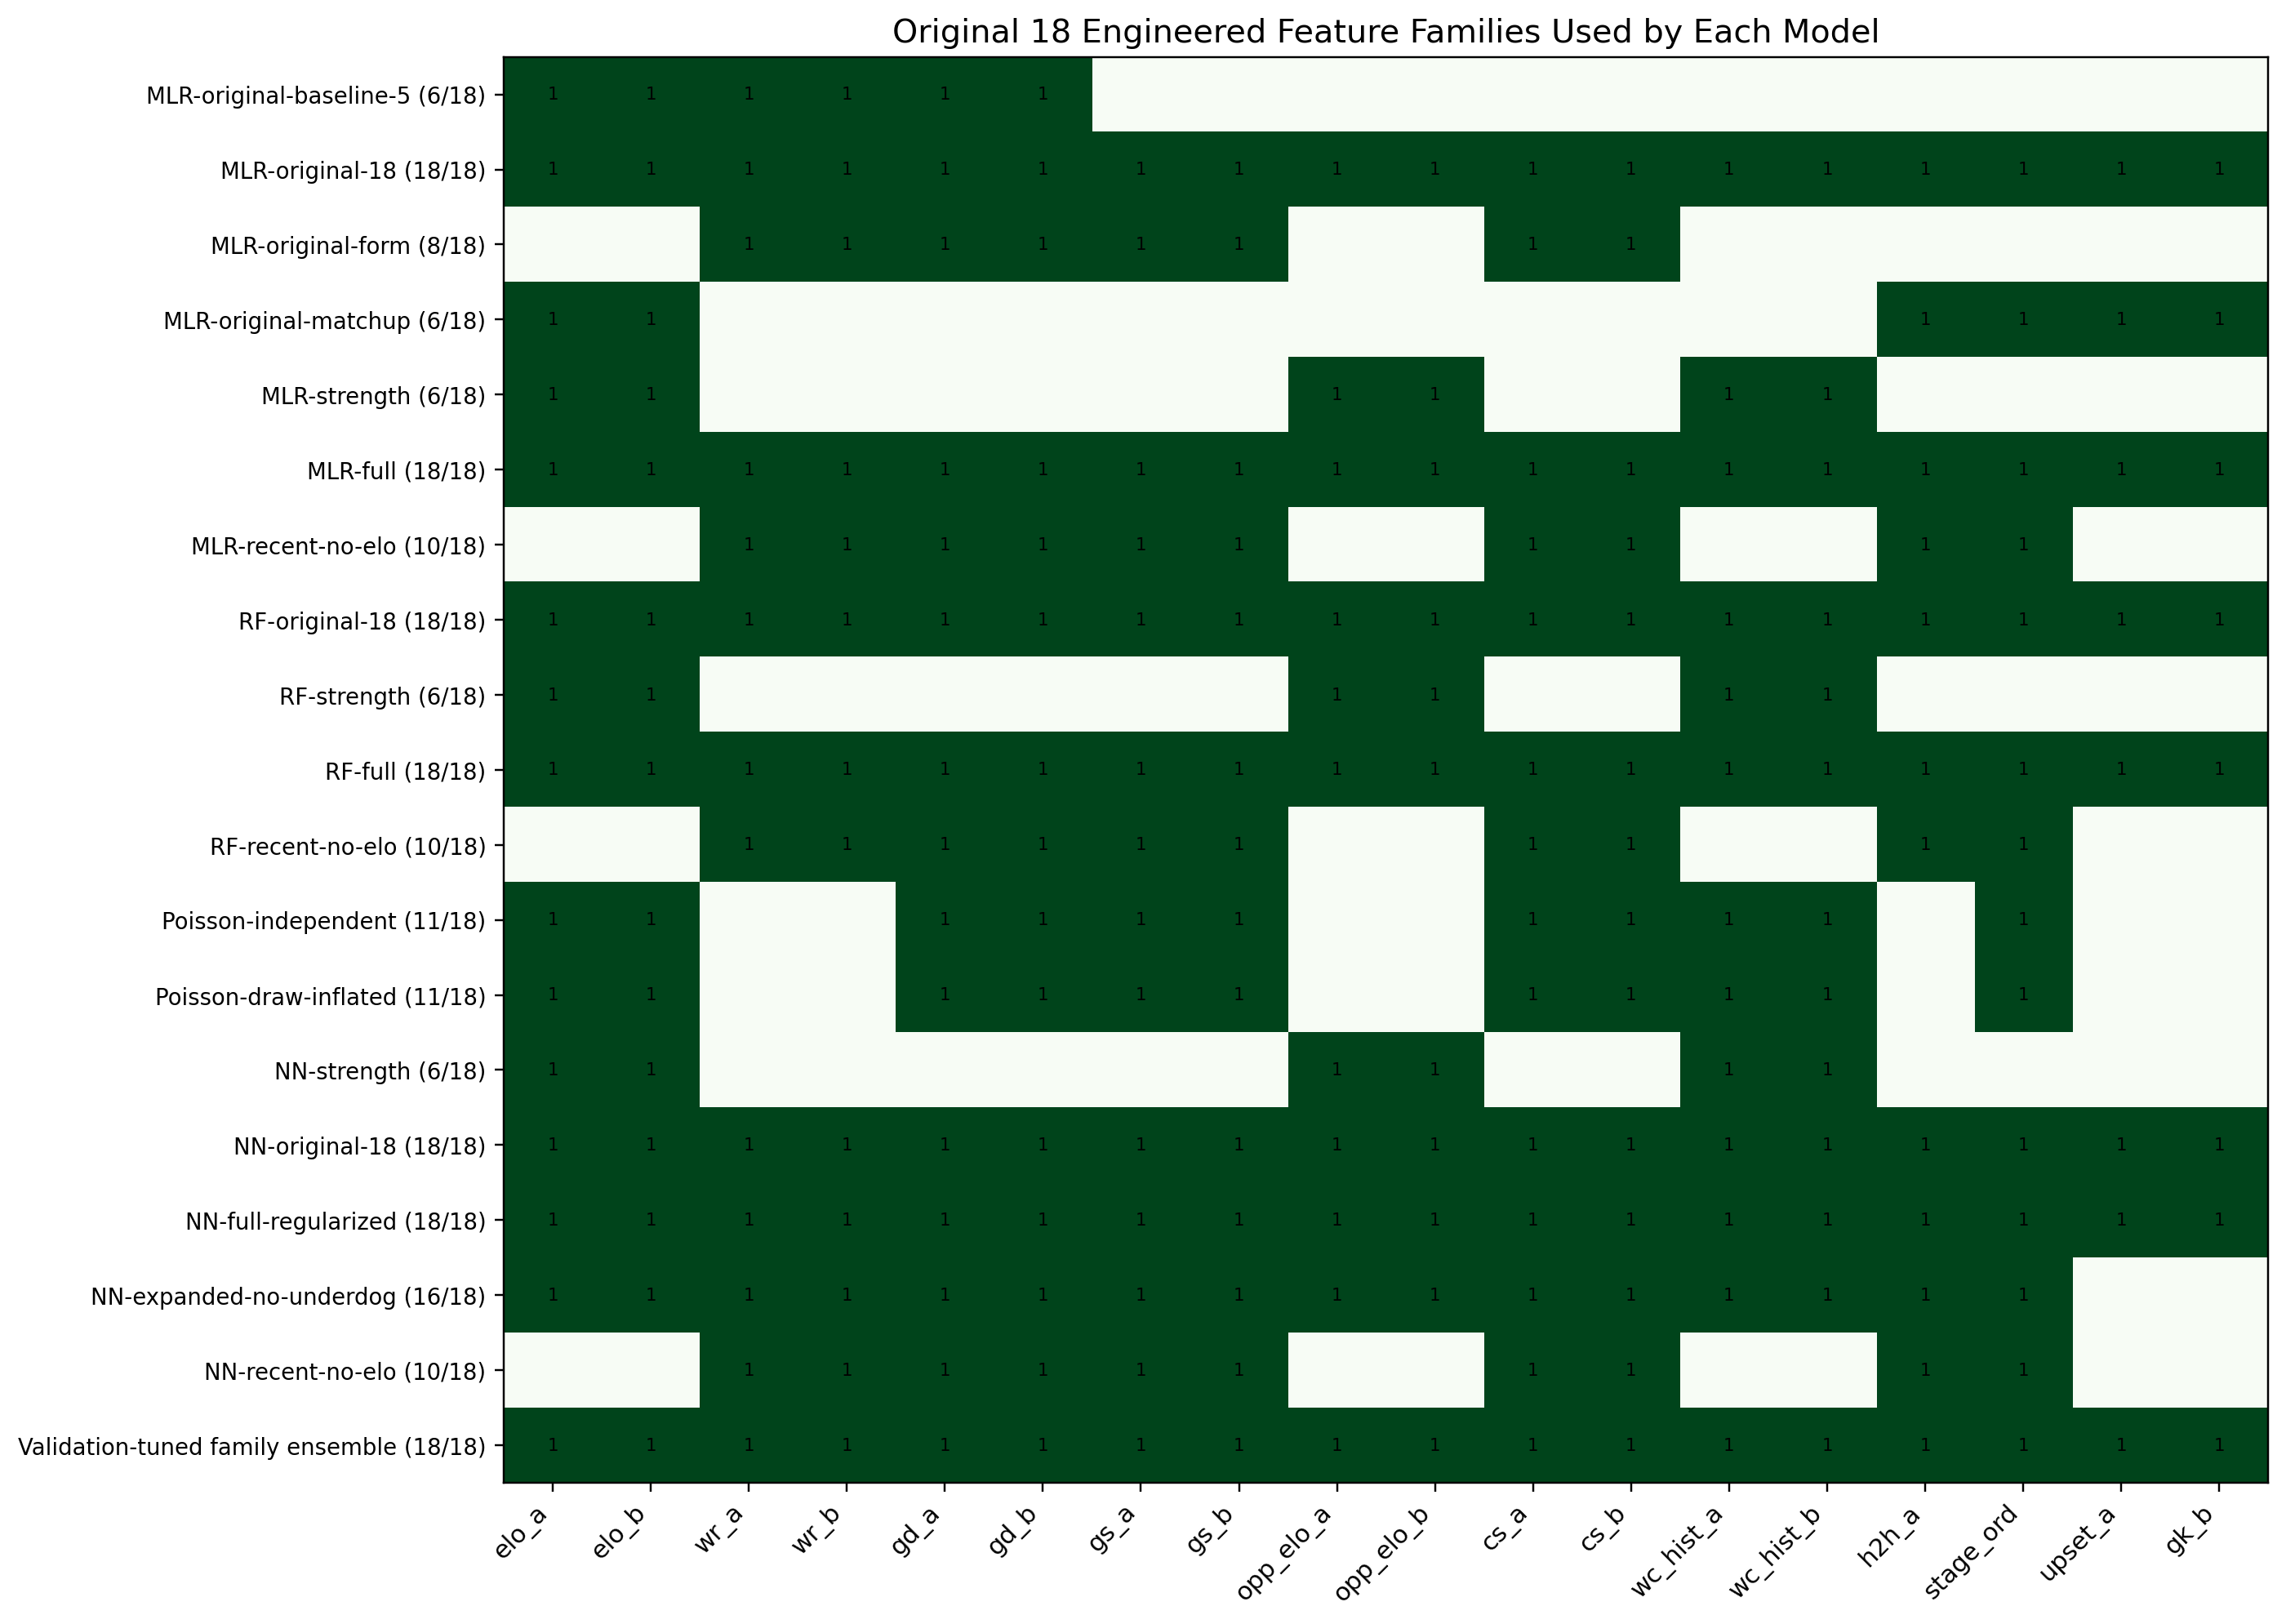
\includegraphics[width=0.97\textwidth]{feature_usage_heatmap.png}
  \caption{Feature-family usage by model. The original 18-feature models use
  all 18 directly; the expanded full MLR/RF/NN models use all 18 through
  55 direct columns.}
  \label{fig:featureusage}
\end{figure}

\paragraph{Model variants.}
We retrain the original MLR feature sets under the new checkpoint protocol:
baseline-5, original-18, form-only, and matchup-only. We also train expanded
MLR, RF, and NN variants: strength, full, and recent-no-Elo. The NN family
adds an original-18 model and a 53-feature no-underdog ablation that removes
\texttt{upset\_a} and \texttt{gk\_b}. Score models include independent Poisson
regression and a draw-inflated Poisson variant. The ensemble chooses one model
per family based only on validation checkpoints and tunes convex weights on
those checkpoints.

\paragraph{Knockout draw handling.}
Draws are valid in group matches, but not as final knockout outcomes. The
pipeline explicitly handles this in two places. During validation and testing,
if a row is a knockout stage, predicted draw probability is set to zero and
win/loss probabilities are renormalized. During 2026 simulation, knockout
score grids are calibrated after setting draw probability to zero, so sampled
knockout scorelines are decisive; a stochastic tiebreak fallback remains for
numerical edge cases. This includes the 2026 round of 32.

\section{Experiments}

Table~\ref{tab:results} reports the final held-out 2022 results after
retraining on all feasible World Cup checkpoints. The best log loss is
NN-original-18 at 0.9321, which is useful because it shows the original
feature set becomes competitive once the training target includes all
international matches. The best hard accuracy is still the
NN-expanded-no-underdog ablation at 60.9\%, with 0.9363 log loss and 30\%
draw recall.

\begin{table}[ht]
\centering
\scriptsize
\caption{Final model comparison. CV summarizes 19 walk-forward World Cup
checkpoints from 1938 through 2018; test is the held-out 2022 World Cup.}
\label{tab:results}
\resizebox{\textwidth}{!}{%
\begin{tabular}{llrrrrrrr}
\toprule
Model & Family & Feat. & Orig. 18 & CV LL & CV Acc & Test LL & Test Acc & Draw Rec. \\
\midrule
NN-original-18 & NN & 18 & 18 & 0.9657 & 0.5133 & \textbf{0.9321} & 0.5156 & 0.0000 \\
NN-full-regularized & NN & 55 & 18 & 0.9630 & 0.4832 & 0.9330 & 0.5312 & 0.0000 \\
MLR-original-18 & MLR & 18 & 18 & 1.0183 & 0.4485 & 0.9340 & 0.4844 & 0.0000 \\
Validation-tuned ensemble & Ensemble & 70 & 18 & \textbf{0.9360} & \textbf{0.5553} & 0.9343 & 0.5469 & 0.0000 \\
NN-strength & NN & 8 & 6 & 0.9739 & 0.4566 & 0.9360 & 0.5000 & 0.0000 \\
NN-expanded-no-underdog & NN & 53 & 16 & 0.9646 & 0.5188 & 0.9363 & \textbf{0.6094} & \textbf{0.3000} \\
NN-recent-no-elo & NN & 28 & 10 & 0.9906 & 0.4712 & 0.9418 & 0.5000 & 0.0000 \\
RF-original-18 & RF & 18 & 18 & 0.9991 & 0.4419 & 0.9475 & 0.5000 & 0.0000 \\
Poisson-independent & Poisson & 13 & 11 & 0.9526 & 0.5387 & 0.9479 & 0.5312 & 0.0000 \\
MLR-full & MLR & 55 & 18 & 1.0409 & 0.4496 & 0.9519 & 0.5312 & 0.1000 \\
Poisson-draw-inflated & Poisson & 13 & 11 & 0.9538 & 0.5367 & 0.9527 & 0.5312 & 0.0000 \\
MLR-recent-no-elo & MLR & 28 & 10 & 1.0337 & 0.4156 & 0.9546 & 0.4844 & 0.2000 \\
MLR-original-matchup & MLR & 6 & 6 & 1.0344 & 0.4261 & 0.9559 & 0.5312 & 0.0000 \\
RF-full & RF & 55 & 18 & 0.9926 & 0.4507 & 0.9562 & 0.5625 & 0.0000 \\
RF-recent-no-elo & RF & 28 & 10 & 1.0073 & 0.4475 & 0.9602 & 0.4844 & 0.1000 \\
MLR-strength & MLR & 8 & 6 & 1.0244 & 0.4297 & 0.9613 & 0.5312 & 0.1000 \\
MLR-original-form & MLR & 8 & 8 & 1.0193 & 0.4455 & 0.9637 & 0.4844 & 0.0000 \\
MLR-original-baseline-5 & MLR & 5 & 6 & 1.0002 & 0.4442 & 0.9651 & 0.5469 & 0.1000 \\
RF-strength & RF & 8 & 6 & 1.0115 & 0.4027 & 0.9702 & 0.5312 & 0.0000 \\
\bottomrule
\end{tabular}}
\end{table}

\begin{figure}[ht]
  \centering
  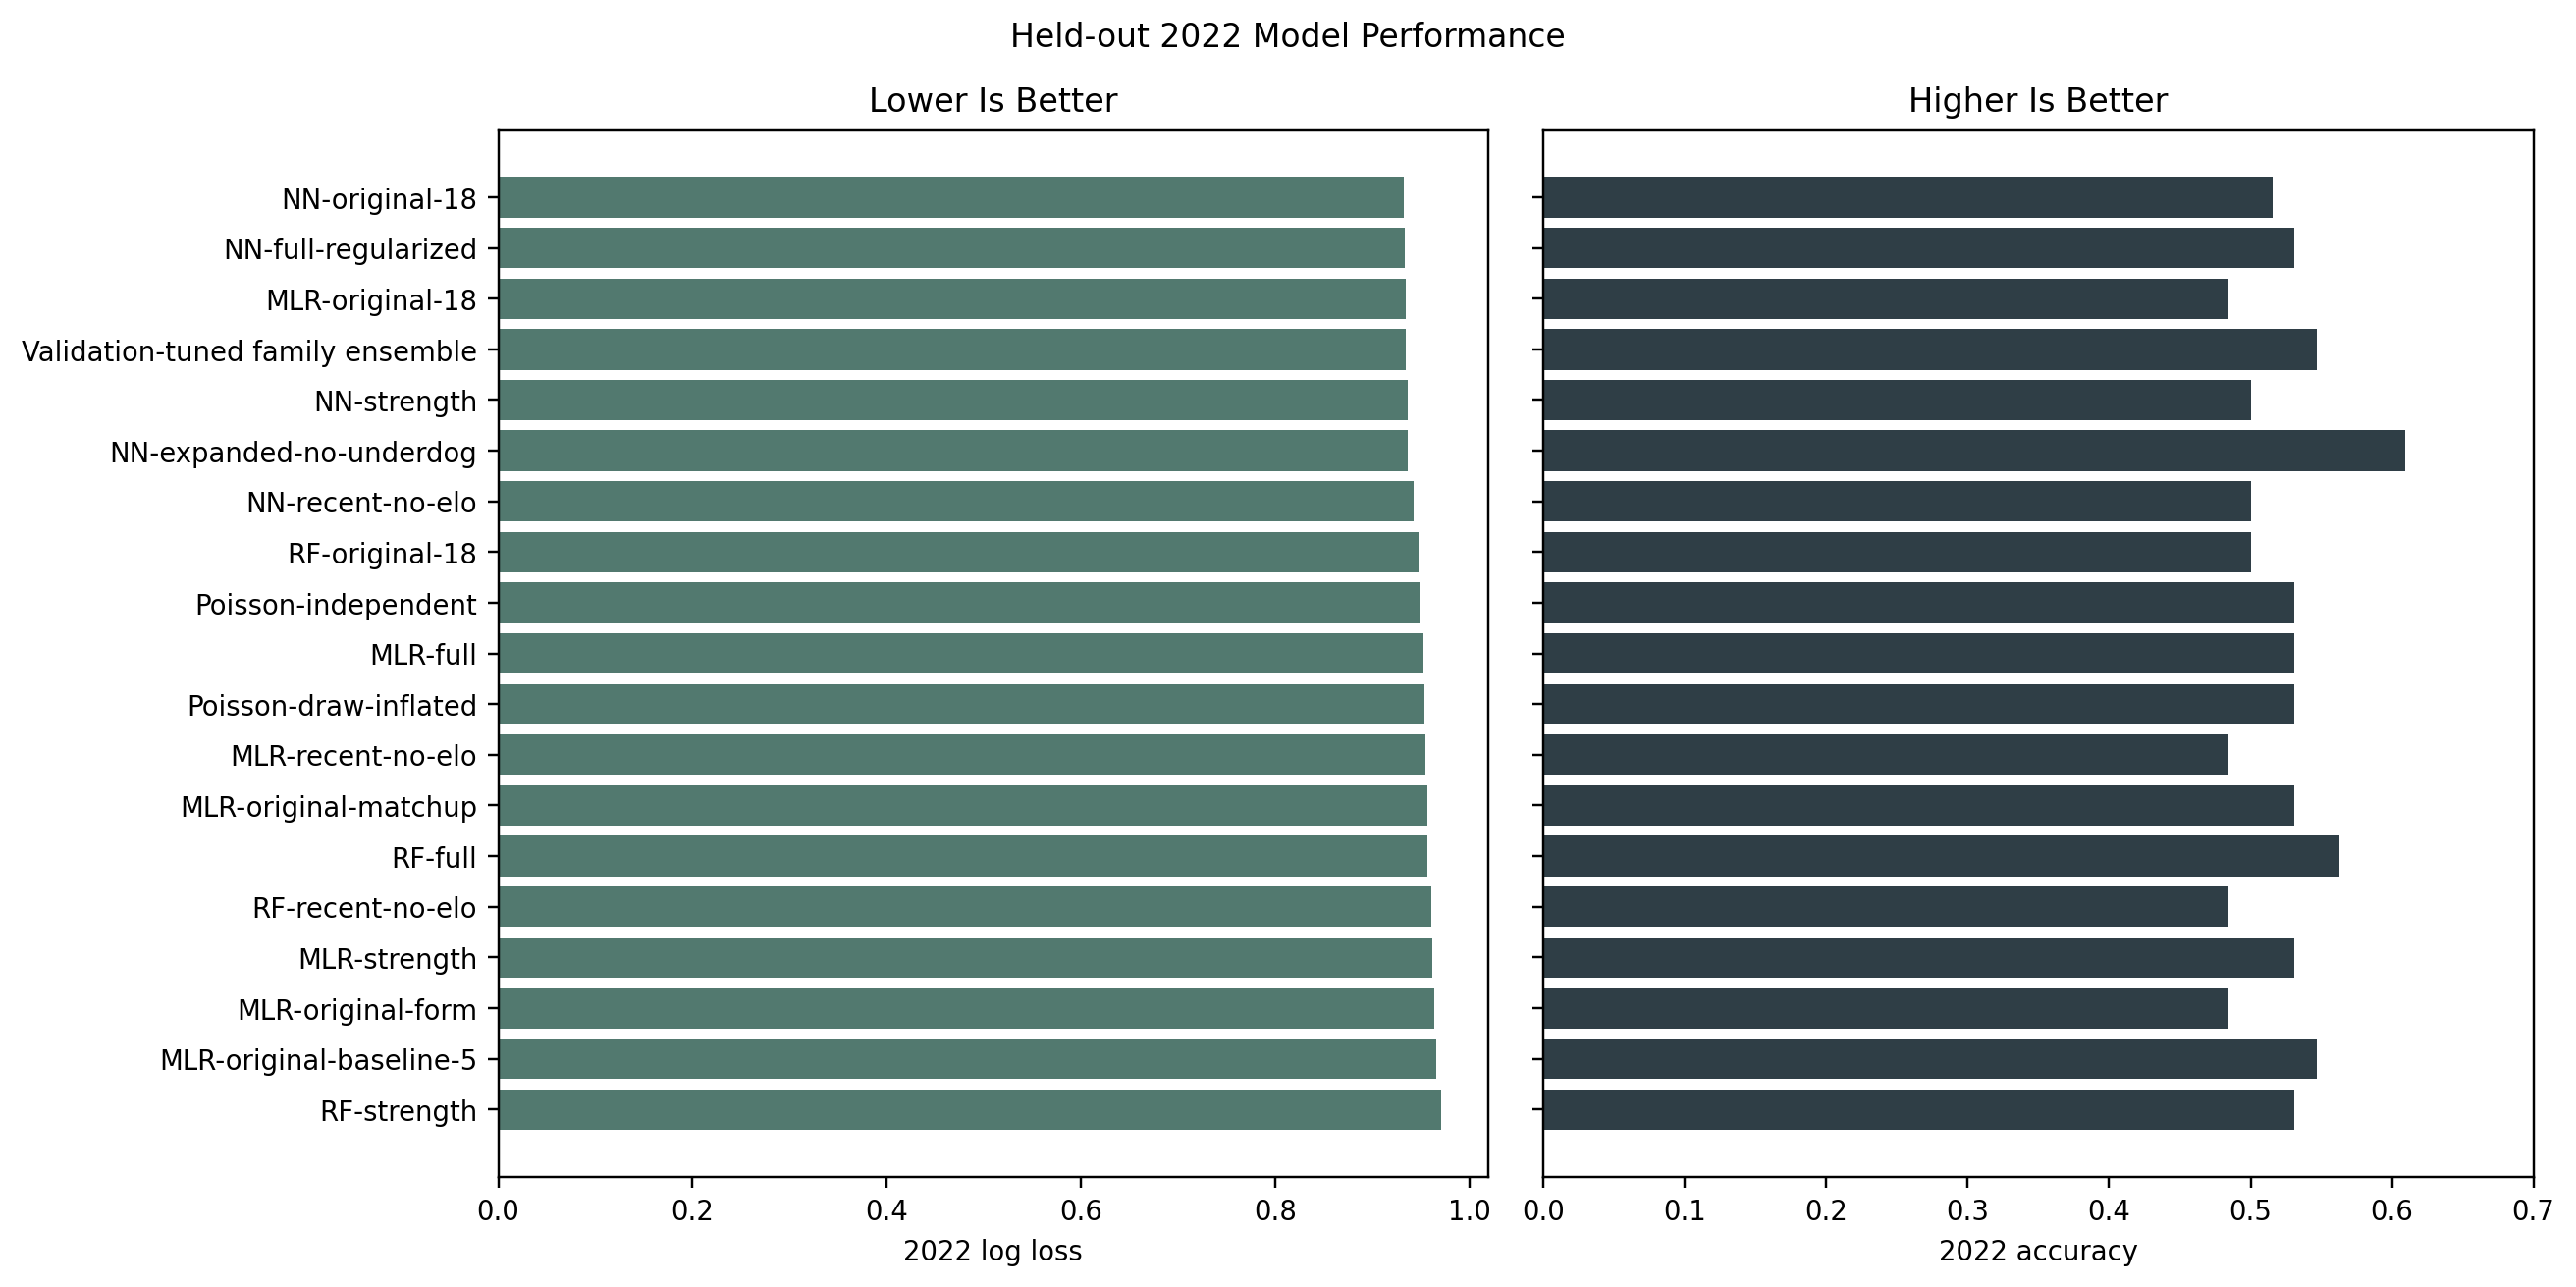
\includegraphics[width=0.93\textwidth]{model_test_metrics.png}
  \caption{Held-out 2022 performance across trained models.}
  \label{fig:testmetrics}
\end{figure}

\begin{figure}[ht]
  \centering
  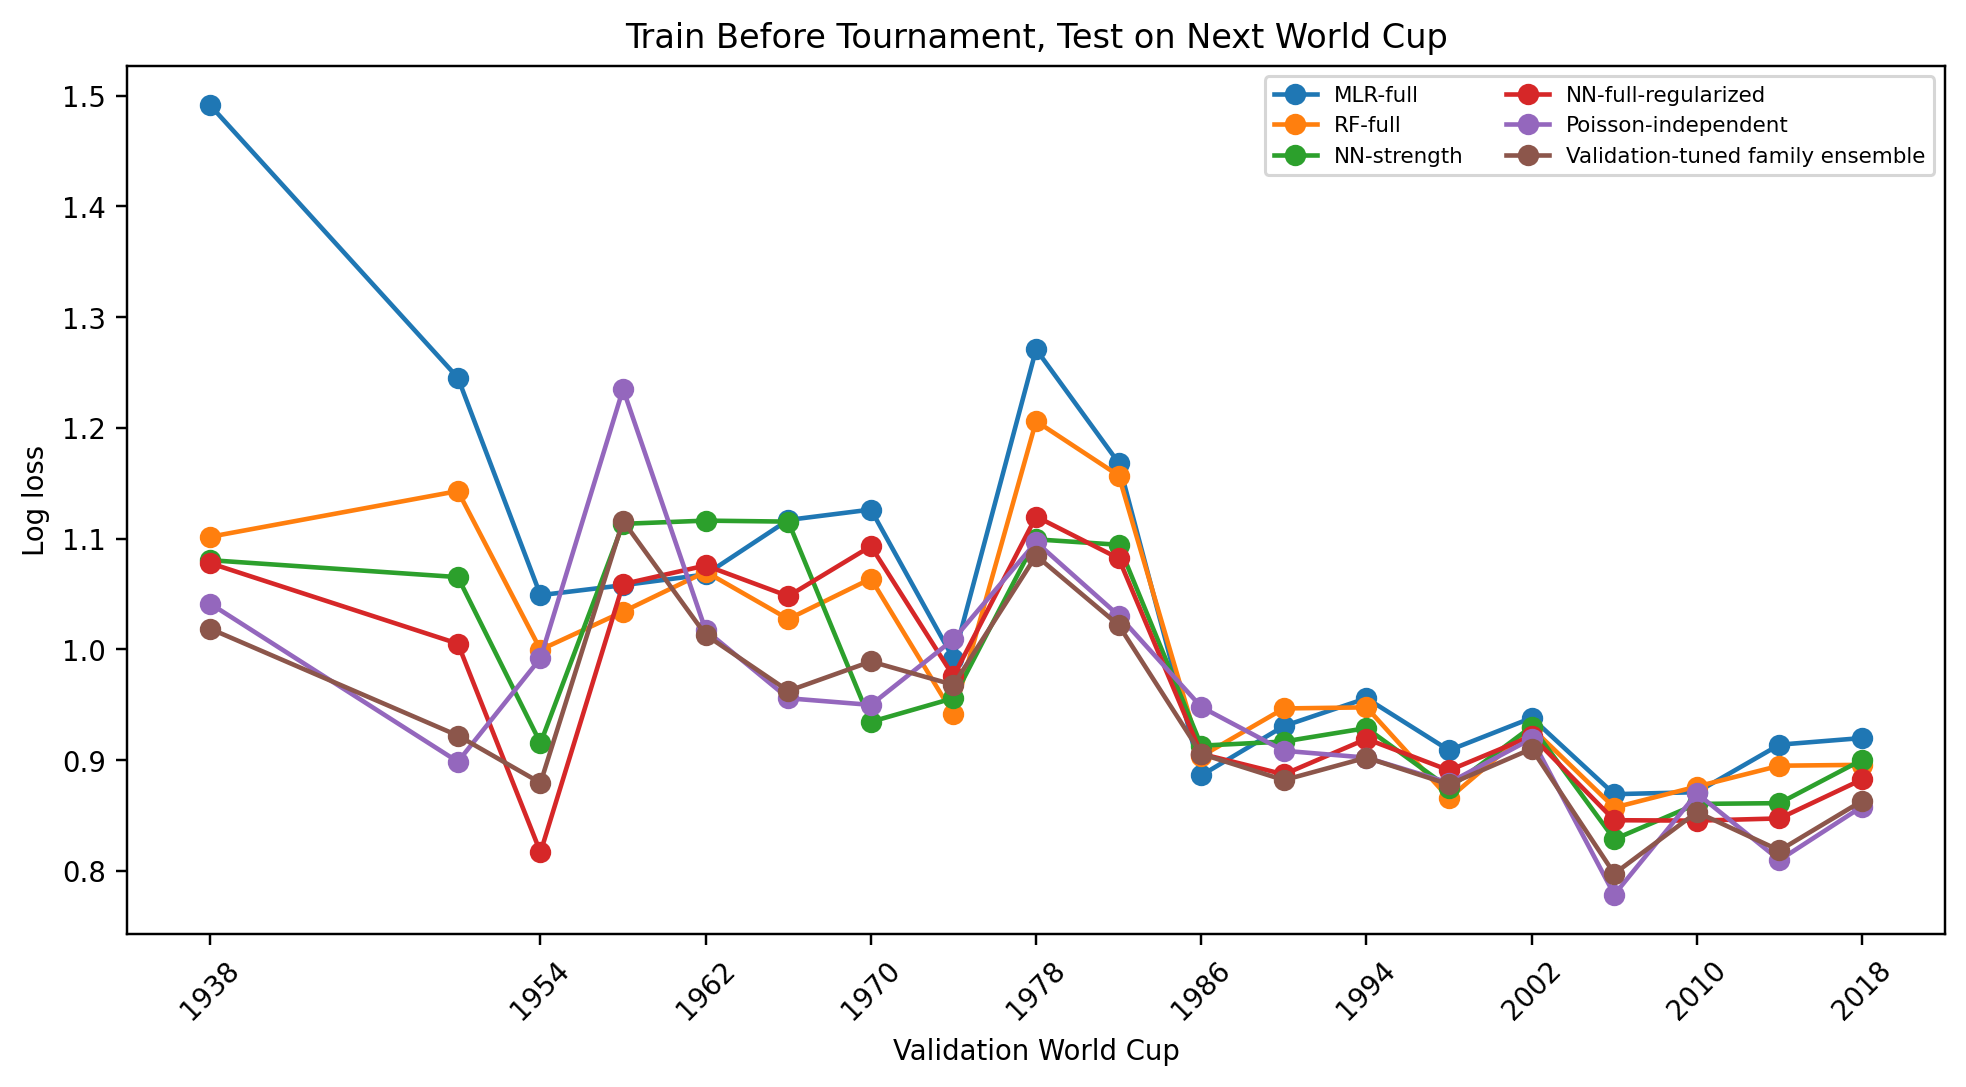
\includegraphics[width=0.82\textwidth]{fold_log_loss.png}
  \caption{Walk-forward log loss by checkpoint. Each point trains before a
  World Cup and validates on that next World Cup.}
  \label{fig:foldll}
\end{figure}

\paragraph{What succeeds and fails.}
The NN family succeeds because supervised international labels provide enough
examples for nonlinear models. The 18-feature NN has the best 2022 log loss,
while the 53-feature NN has the best 2022 accuracy. This is the central
accuracy-vs-log-loss tradeoff introduced in Section 1: the best calibrated
probability model is not the best hard classifier. Figure~\ref{fig:foldll}
shows why we report both metrics. Per-checkpoint log loss moves substantially
across eras because tournament size, draw rates, and international data
coverage change; a single average would hide this instability. MLR is stable
but underfits nonlinear context, RF trails on log loss because tree
probabilities are less smooth on small folds, and Poisson models are useful
for simulation because they generate score distributions even when their
argmax predictions rarely select draws.

\begin{table}[ht]
\centering
\small
\caption{Representative 2022 confusion matrices. Rows are actual labels and
columns are predicted labels.}
\label{tab:confusions}
\begin{tabular}{llrrr}
\toprule
Model & Actual & Pred W & Pred D & Pred L \\
\midrule
\multirow{3}{*}{NN-original-18} & W & 27 & 0 & 6 \\
 & D & 7 & 0 & 3 \\
 & L & 15 & 0 & 6 \\
\midrule
\multirow{3}{*}{NN-expanded-no-underdog} & W & 30 & 0 & 3 \\
 & D & 6 & 3 & 1 \\
 & L & 15 & 0 & 6 \\
\midrule
\multirow{3}{*}{Poisson-independent} & W & 32 & 0 & 1 \\
 & D & 10 & 0 & 0 \\
 & L & 18 & 0 & 3 \\
\bottomrule
\end{tabular}
\end{table}

\section{2026 Forecast}

The 2026 World Cup forecast uses a hybrid outcome/score simulator. The primary
simulator uses NN-original-18, the best held-out log-loss model, for W/D/L
probabilities. It separately fits a Poisson goal layer, then reweights the
score grid so the total win/draw/loss mass matches the NN probabilities. This
keeps the calibrated classifier in charge of match outcomes while still
producing goals for group points, goal difference, goals for, and knockout
advancement. Model selection uses only the historical
validation checkpoints, but the final 2026 fit uses an augmented table of
19,239 rows: the original 14,881 rows plus 4,358 post-cache international
matches from 2022 through March 31, 2026. These rows also update Elo and
rolling-form state before the tournament simulation. The simulator reads the
group field from \texttt{config/2026\_groups.csv}, advances the top two teams
in each group plus the eight best third-place teams, and then uses a
transparent high-vs-low seeded knockout approximation. This approximation is
reproducible but does not fully encode FIFA's exact round-of-32 pairing table.

\begin{figure}[t]
  \centering
  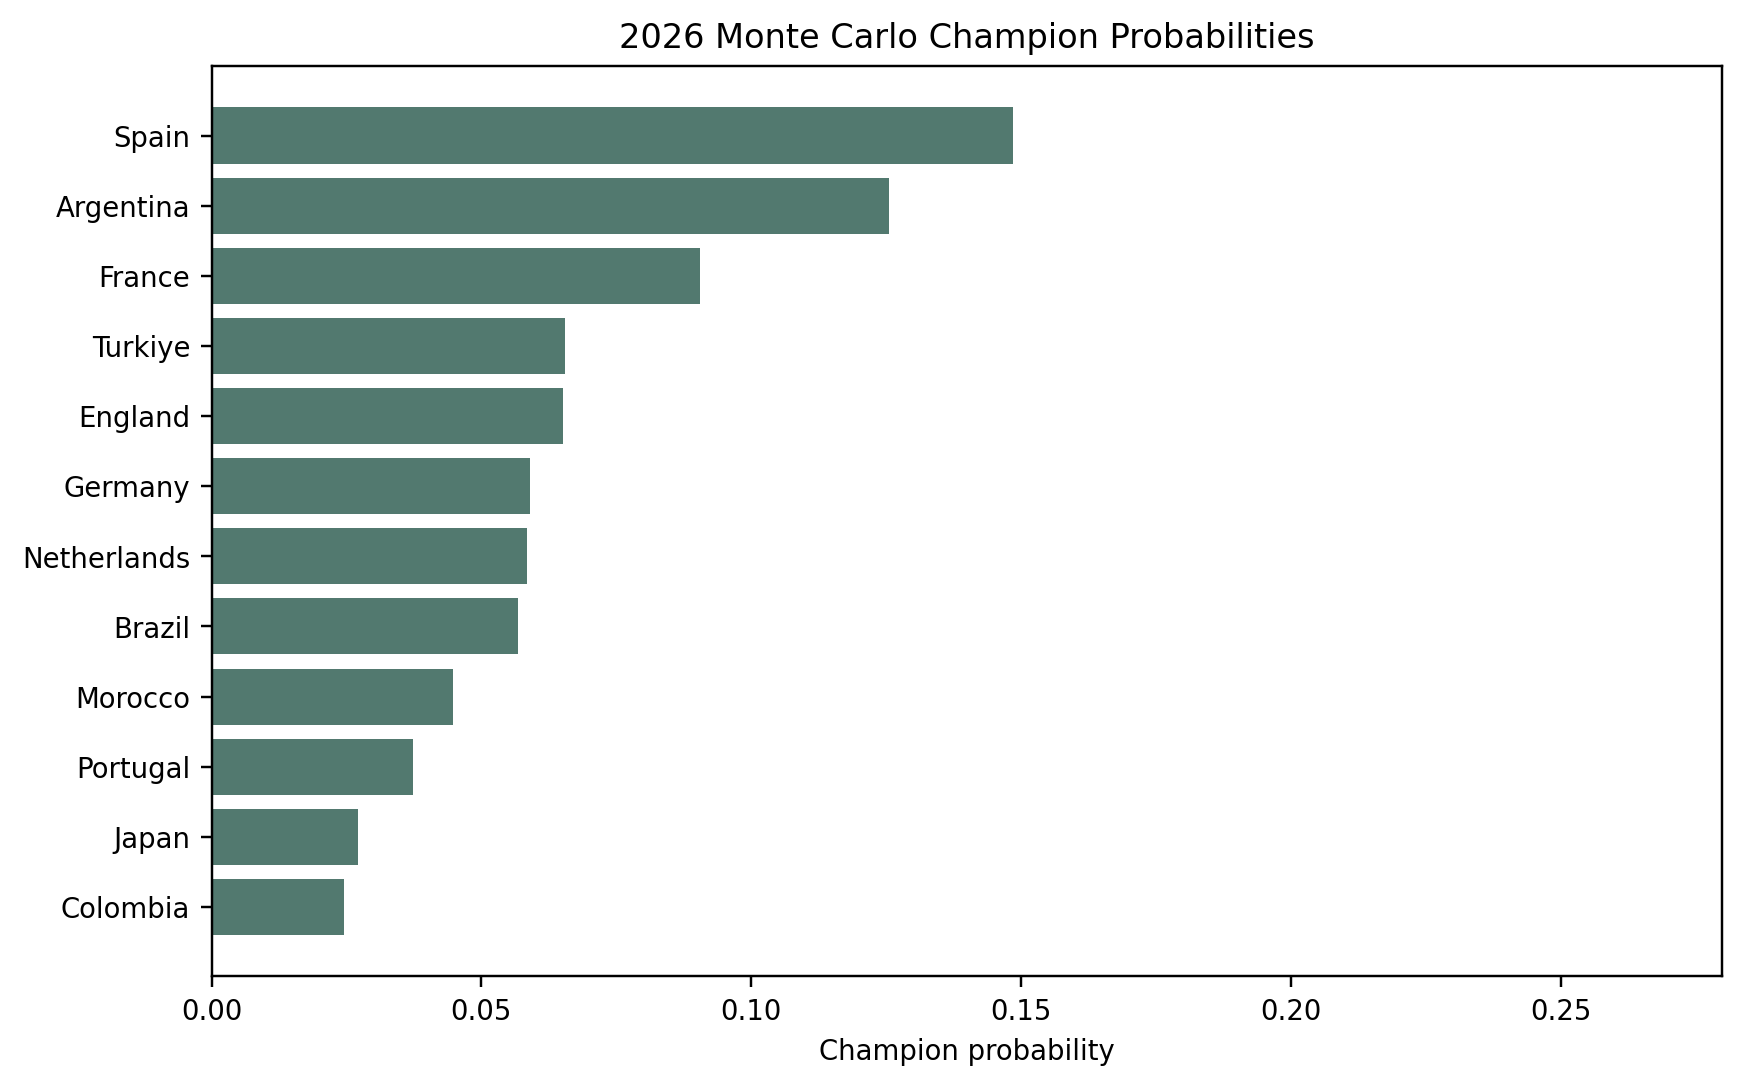
\includegraphics[width=0.70\textwidth]{champion_probabilities_2026.png}
  \caption{Top 2026 champion probabilities from 5,000 Monte Carlo simulations.}
  \label{fig:champions}
\end{figure}

The top primary championship probabilities are Spain 14.9\%, Argentina
12.6\%, France 9.1\%, Turkiye 6.5\%, England 6.5\%, Germany 5.9\%,
Netherlands 5.8\%, Brazil 5.7\%, Morocco 4.5\%, and Portugal 3.7\%. Polymarket
placed Spain at 15.3\% in the April 30, 2026 snapshot
\citep{polymarket2026odds}, so the primary model is close to the market's
Spain estimate while assigning more probability to Argentina and less to
France, England, Brazil, and Portugal. For sensitivity, the appendix reports
all 48 champion probabilities for four forecast variants: Poisson-only, the
primary NN-original-18 hybrid, the high-accuracy NN hybrid, and the
validation-tuned ensemble hybrid. The spread across variants shows that winner
forecasts are more model-sensitive than the 2022 W/D/L test metrics alone
suggest.

\section{Related Work}

Football score prediction often begins with Poisson goal models
\citep{maher1982modelling}. Dixon and Coles improve this family by correcting
low-score dependence \citep{dixon1997modelling}. Elo ratings are effective
features for football outcome prediction \citep{hvattum2010using}. Random
forests and hybrid tournament models have also been applied to international
football \citep{schauberger2018predicting,groll2019hybrid}. Tournament
simulators commonly combine match probabilities with Monte Carlo brackets
\citep{groll2015prediction,fivethirtyeight2022}. Our contribution is the
course-project system design: all supervised international labels,
walk-forward World Cup checkpoints, multiple model families, feature-family
accounting, and a reproducible classifier-calibrated 2026 simulation.

\newpage
\section{Discussion}

The project satisfies the main technical goals: it compares MLR, RF, NN, and
Poisson variants; reports accuracy and log loss; uses all feasible World Cup
checkpoints; and produces a full 2026 forecast. The strongest lesson is that
model capacity only helps when the training target contains enough supervised
labels. Here, the NN models are viable because they train on thousands of
international matches while still validating on future World Cups. The broader
implication is that sports prediction papers
should avoid a single ``best model'' claim: calibrated probabilities and hard
classification can favor different models, and tournament-era variability
should be shown rather than averaged away.

The remaining limitations are concrete. First, the 2026-only supplement
improves freshness but still lacks squad availability, injuries, roster depth,
and market information. Second, the knockout bracket is approximated rather
than exact. Third, the models still struggle with draws: the best accuracy NN
predicts some 2022 draws, but most families do not. A production version
should keep the 2022--2026 match feed current through the tournament, add
official rankings and squad availability, calibrate probabilities explicitly,
and encode the exact 2026 bracket. The submitted directory is self-contained,
and the report stands alone as a complete description of the project.

\clearpage
\bibliographystyle{plainnat}
\bibliography{bibliography}

\clearpage
\appendix

\section{Additional Figures and Tables}

\begin{figure}[ht]
  \centering
  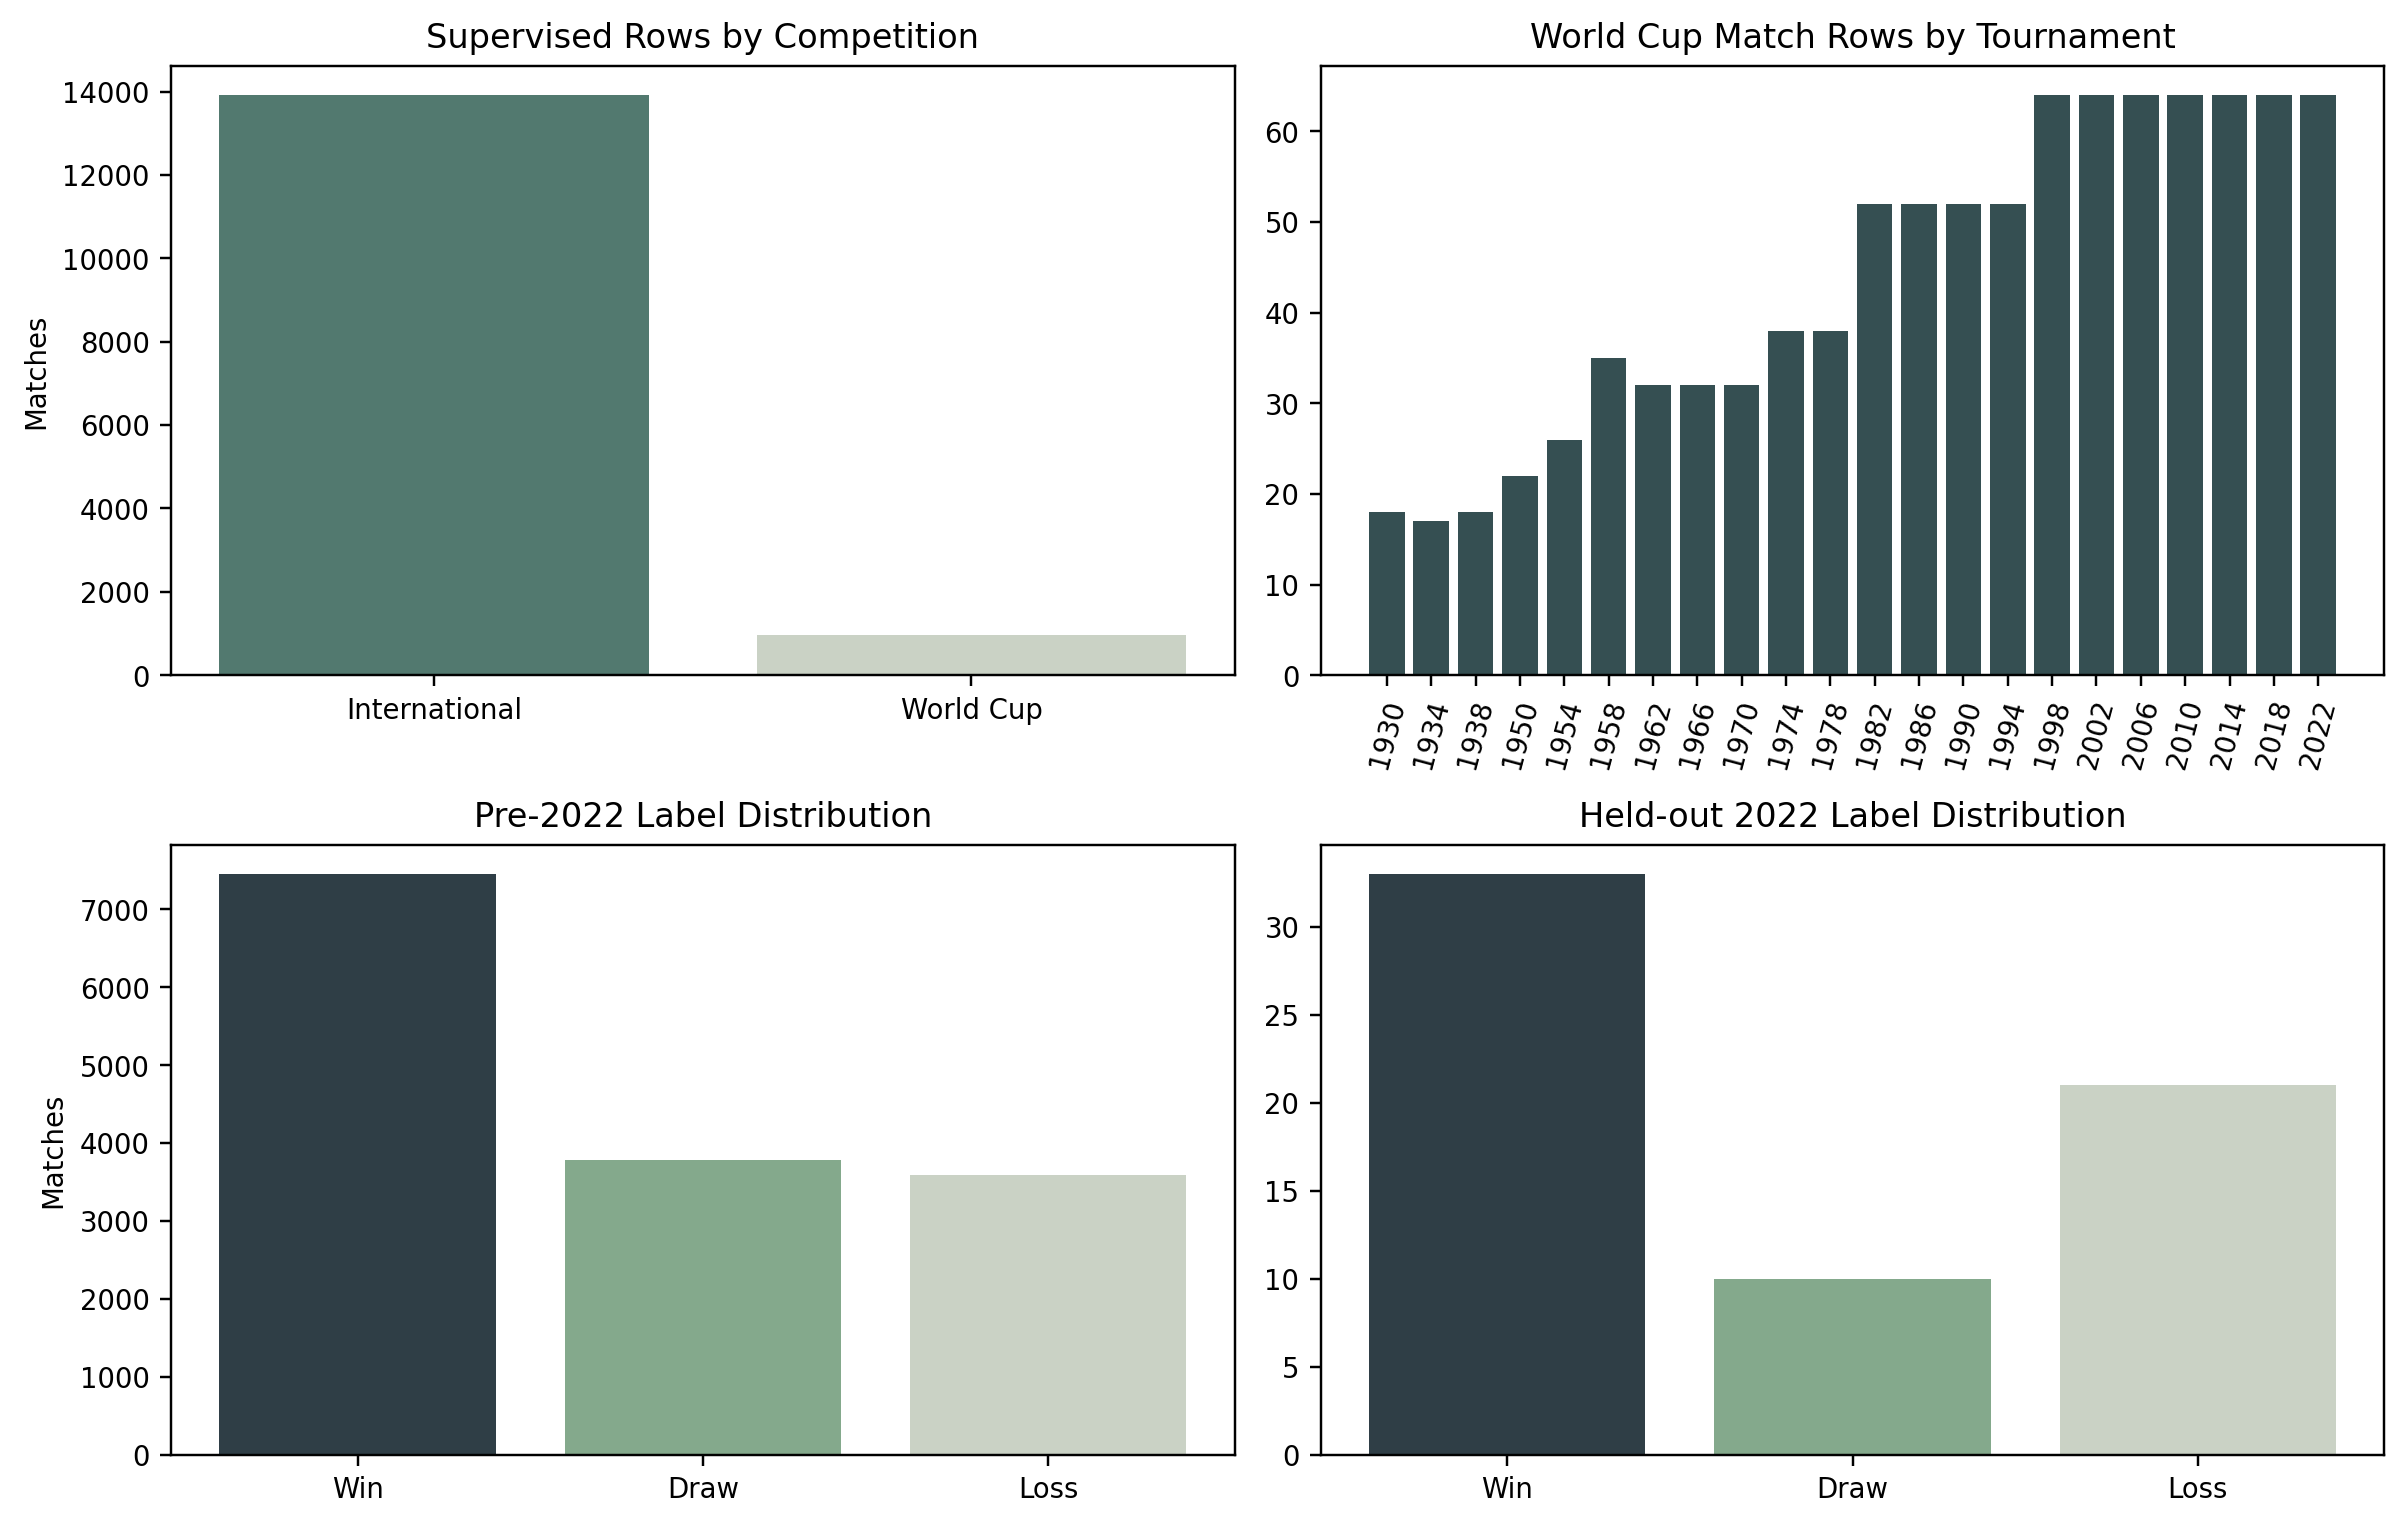
\includegraphics[width=\textwidth]{dataset_overview.png}
  \caption{Dataset overview used by the final pipeline.}
  \label{fig:datasetappendix}
\end{figure}

\begin{figure}[ht]
  \centering
  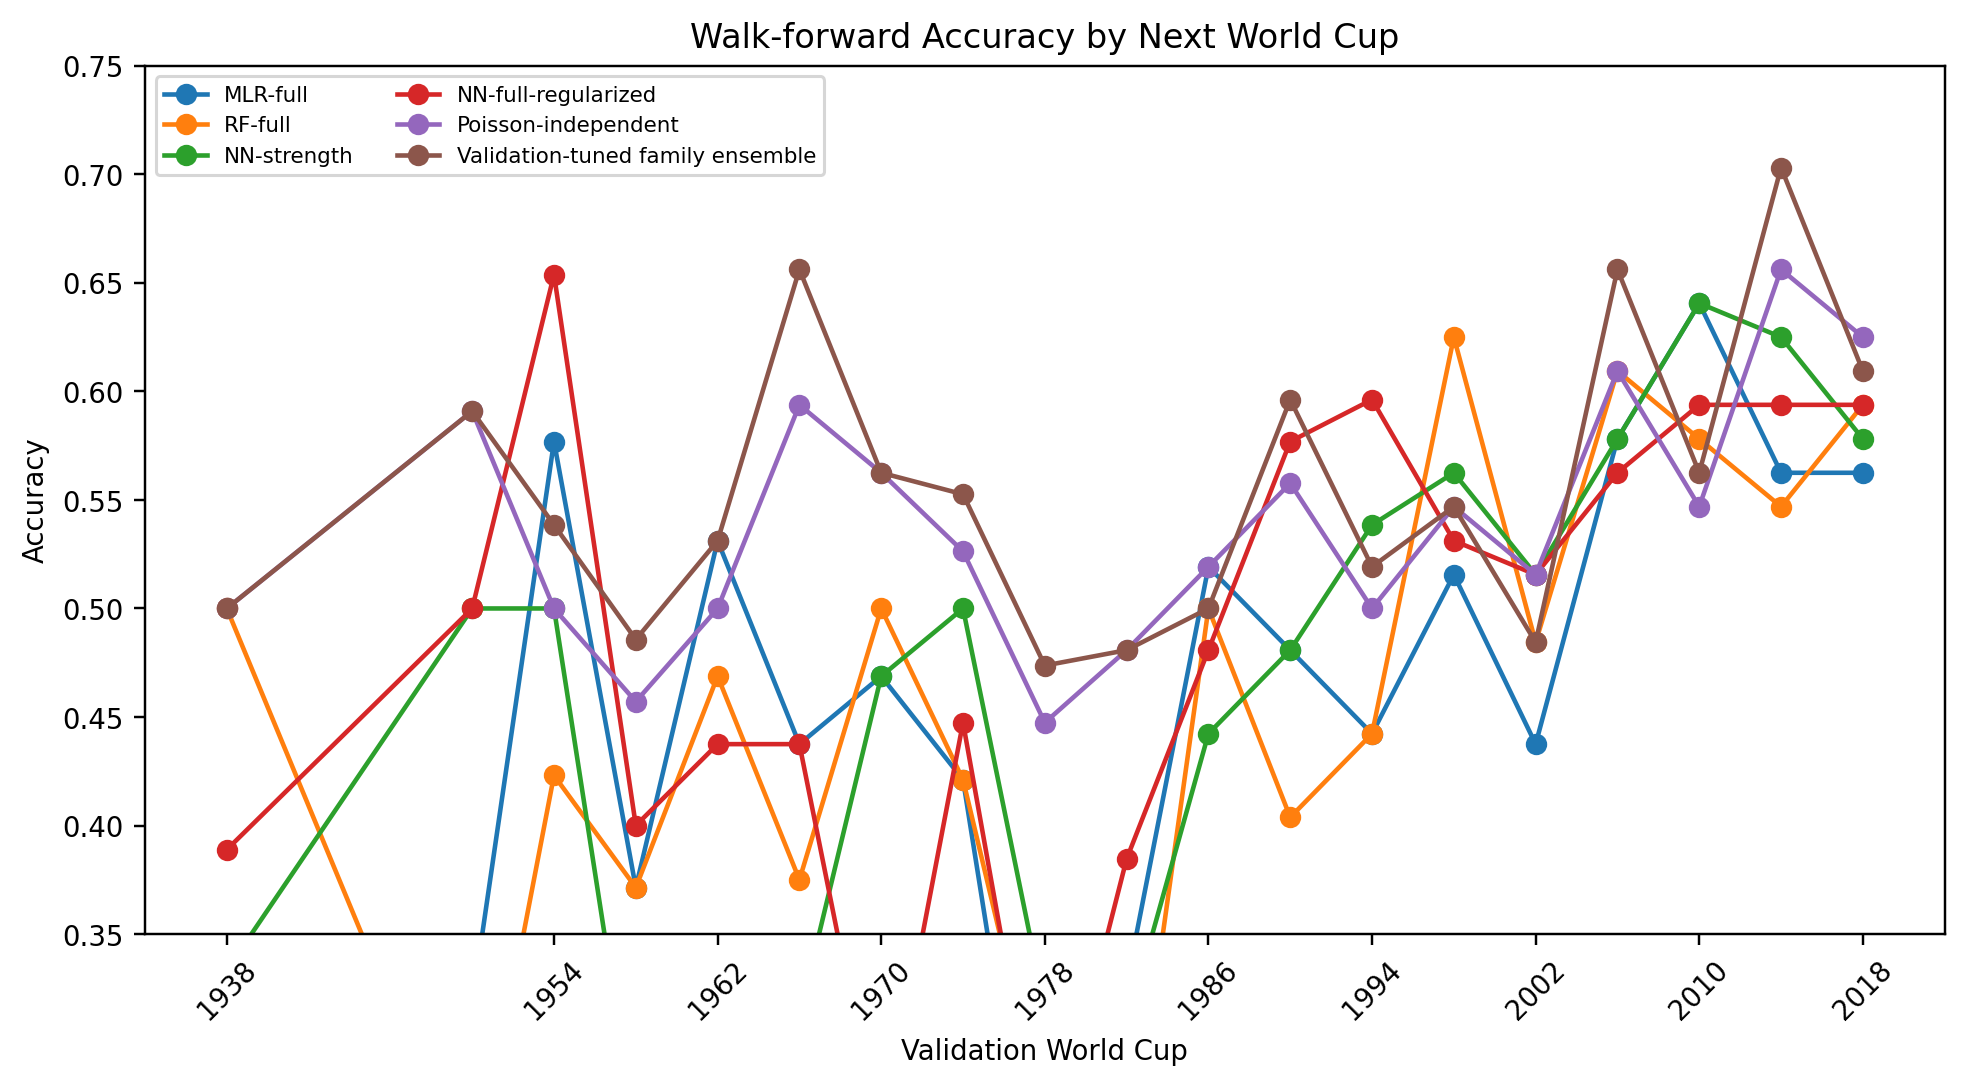
\includegraphics[width=0.94\textwidth]{fold_accuracy.png}
  \caption{Walk-forward accuracy by validation World Cup.}
  \label{fig:foldacc}
\end{figure}

\begin{figure}[ht]
  \centering
  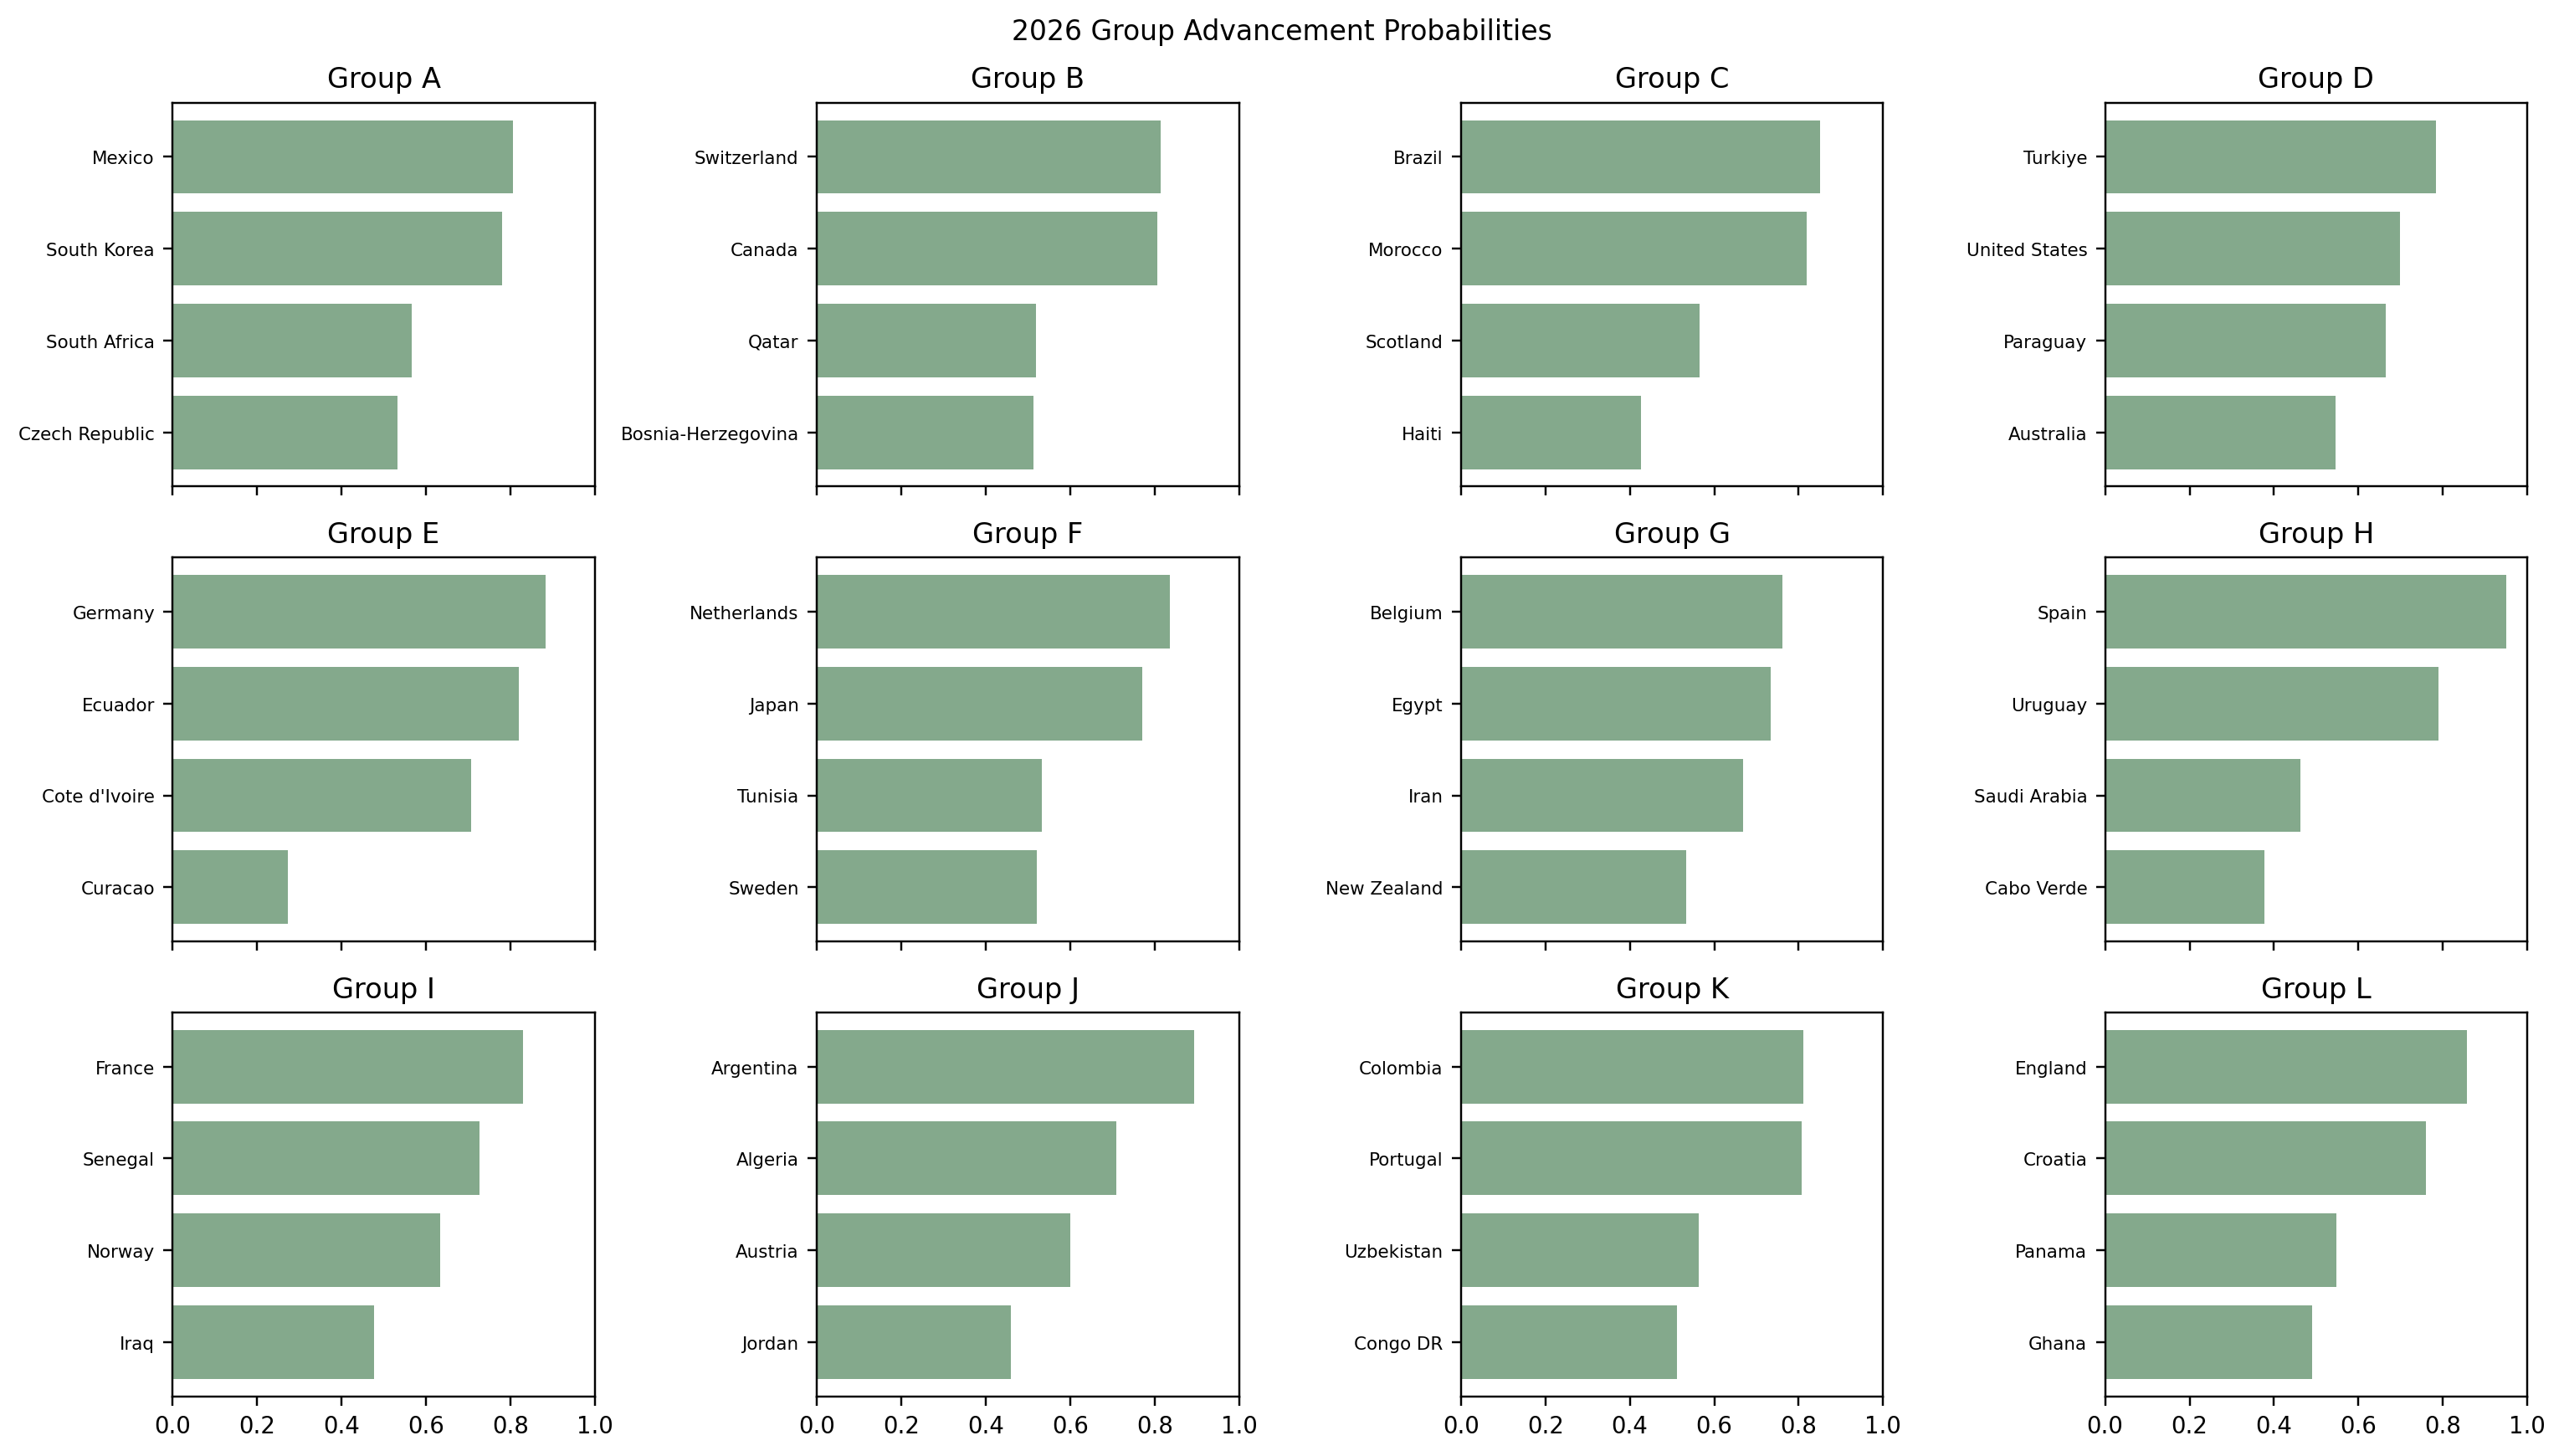
\includegraphics[width=\textwidth]{group_advancement_2026.png}
  \caption{Simulated group advancement probabilities for the configured 2026
  group field.}
  \label{fig:groupadv}
\end{figure}

\begin{table}[p]
\centering
\scriptsize
\setlength{\tabcolsep}{3pt}
\renewcommand{\arraystretch}{0.92}
\caption{2026 champion probabilities for every forecast simulator, compared
with Polymarket implied winner probabilities from the April 30, 2026 market
snapshot \citep{polymarket2026odds}. Values are percentages. NN18 is the
primary NN-original-18 calibrated score simulator; NN53 is the high-accuracy
NN-expanded-no-underdog calibrated score simulator.}
\label{tab:forecastvariants}
\begin{tabular}{lrrrrr}
\toprule
Team & Poisson & NN18 & NN53 & Ensemble & Polymarket \\
\midrule
Spain & 25.1 & 14.9 & 14.8 & 19.1 & 15.3 \\
Argentina & 19.7 & 12.6 & 9.0 & 15.0 & 8.7 \\
France & 13.0 & 9.1 & 6.7 & 9.6 & 16.4 \\
Turkiye & 2.6 & 6.5 & 2.7 & 3.5 & 0.7 \\
England & 6.9 & 6.5 & 7.0 & 6.6 & 11.1 \\
Germany & 4.1 & 5.9 & 4.7 & 4.9 & 5.2 \\
Netherlands & 4.3 & 5.8 & 4.1 & 5.4 & 3.4 \\
Brazil & 1.4 & 5.7 & 4.4 & 3.3 & 8.6 \\
Morocco & 4.8 & 4.5 & 5.5 & 4.0 & 1.9 \\
Portugal & 3.0 & 3.7 & 3.8 & 3.2 & 7.4 \\
Japan & 3.7 & 2.7 & 3.8 & 3.5 & 2.2 \\
Colombia & 1.0 & 2.5 & 3.3 & 2.0 & 1.7 \\
Mexico & 1.4 & 2.3 & 2.3 & 2.2 & 1.1 \\
Belgium & 0.8 & 1.6 & 1.0 & 1.5 & 2.0 \\
Switzerland & 0.5 & 1.6 & 1.9 & 1.1 & 1.0 \\
Croatia & 1.4 & 1.6 & 2.1 & 1.8 & 1.1 \\
Uruguay & 0.2 & 1.3 & 1.4 & 0.9 & 1.1 \\
Ecuador & 1.7 & 1.2 & 3.7 & 1.4 & 0.8 \\
Senegal & 0.6 & 1.0 & 1.6 & 1.3 & 0.8 \\
Algeria & 0.4 & 1.0 & 1.0 & 0.7 & 0.4 \\
Paraguay & 0.2 & 0.8 & 1.2 & 0.7 & 0.5 \\
Iran & 0.5 & 0.8 & 1.2 & 1.1 & 0.2 \\
Canada & 0.3 & 0.8 & 1.1 & 0.9 & 0.7 \\
Norway & 0.7 & 0.7 & 1.8 & 1.3 & 2.4 \\
South Korea & 0.4 & 0.7 & 1.3 & 0.9 & 0.5 \\
United States & 0.1 & 0.7 & 1.1 & 0.4 & 1.6 \\
Egypt & 0.1 & 0.6 & 0.7 & 0.4 & 0.5 \\
Cote d'Ivoire & 0.1 & 0.6 & 0.6 & 0.3 & 0.5 \\
Australia & 0.5 & 0.5 & 1.1 & 0.8 & 0.3 \\
Sweden & 0.0 & 0.3 & 0.5 & 0.1 & 0.7 \\
Austria & 0.2 & 0.3 & 0.5 & 0.6 & 0.7 \\
Tunisia & 0.0 & 0.2 & 0.4 & 0.1 & 0.4 \\
Uzbekistan & 0.2 & 0.2 & 0.6 & 0.5 & 0.3 \\
Scotland & 0.0 & 0.1 & 0.4 & 0.2 & 0.4 \\
Panama & 0.1 & 0.1 & 0.5 & 0.3 & 0.3 \\
Haiti & 0.0 & 0.1 & 0.1 & 0.1 & 0.2 \\
Czech Republic & 0.0 & 0.1 & 0.1 & 0.1 & 0.4 \\
South Africa & 0.0 & 0.1 & 0.1 & 0.0 & 0.3 \\
Jordan & 0.0 & 0.1 & 0.5 & 0.0 & 0.3 \\
Congo DR & 0.0 & 0.1 & 0.2 & 0.2 & 0.3 \\
Iraq & 0.0 & 0.1 & 0.3 & 0.1 & 0.3 \\
Ghana & 0.0 & 0.1 & 0.1 & 0.0 & 0.3 \\
Bosnia-Herzegovina & 0.0 & 0.0 & 0.1 & 0.0 & 0.4 \\
Qatar & 0.0 & 0.0 & 0.1 & 0.0 & 0.3 \\
Cabo Verde & 0.0 & 0.0 & 0.1 & 0.0 & 0.3 \\
Curacao & 0.0 & 0.0 & 0.0 & 0.0 & 0.3 \\
New Zealand & 0.0 & 0.0 & 0.4 & 0.1 & 0.3 \\
Saudi Arabia & 0.0 & 0.0 & 0.2 & 0.0 & 0.3 \\
\bottomrule
\end{tabular}
\end{table}

\begin{table}[ht]
\centering
\scriptsize
\caption{Full glossary of the 18 engineered feature families.}
\label{tab:glossary}
\begin{tabularx}{\textwidth}{llX}
\toprule
Feature & Family & Definition \\
\midrule
\texttt{elo\_a} & Strength & Pre-match Elo rating of higher-rated team A. \\
\texttt{elo\_b} & Strength & Pre-match Elo rating of lower-rated team B. \\
\texttt{wr\_a} & Recent form & Team A win-rate over the recent-match form window. \\
\texttt{wr\_b} & Recent form & Team B win-rate over the recent-match form window. \\
\texttt{gd\_a} & Recent form & Team A average goal differential over the form window. \\
\texttt{gd\_b} & Recent form & Team B average goal differential over the form window. \\
\texttt{gs\_a} & Recent attack & Team A average goals scored over the form window. \\
\texttt{gs\_b} & Recent attack & Team B average goals scored over the form window. \\
\texttt{opp\_elo\_a} & Schedule strength & Average recent opponent Elo faced by team A. \\
\texttt{opp\_elo\_b} & Schedule strength & Average recent opponent Elo faced by team B. \\
\texttt{cs\_a} & Recent defense & Team A clean-sheet rate over the form window. \\
\texttt{cs\_b} & Recent defense & Team B clean-sheet rate over the form window. \\
\texttt{wc\_hist\_a} & Tournament history & Time-decayed deepest prior World Cup stage reached by team A. \\
\texttt{wc\_hist\_b} & Tournament history & Time-decayed deepest prior World Cup stage reached by team B. \\
\texttt{h2h\_a} & Matchup & Historical head-to-head score for team A against team B. \\
\texttt{stage\_ord} & Context & Ordinal match-stage indicator from group stage through final. \\
\texttt{upset\_a} & Upset tendency & Exponential moving-average rate at which team A lost matches while favored by Elo. \\
\texttt{gk\_b} & Underdog tendency & Exponential moving-average rate at which team B won matches while unfavored by Elo. \\
\bottomrule
\end{tabularx}
\end{table}

\end{document}
